\chapter{波导}
\label{chap:waveguide}
同轴线可以把任意低频的行波从一端送到另一端，而同样由金属围成的空心矩形管有最低传播频率。两种结构的差别来自导体给横向场施加的边界条件。
本章先求电磁场在金属表面激起的电流和损耗，再由边界条件求波导的模式、截止频率和传输功率。最后将波导两端封闭，考察谐振腔的储能、损耗和品质因子。

\section{导体表面和内部的场}
理想导体(perfect conductor)的零电阻条件给出内部$\bm E = 0$，由Faraday定律只能推出$\p\bm B/\p t = 0$，即初始磁场保持不变。超导体(superconductor)在Meißner态还会排斥体内磁场（表面穿透层除外），因此零电阻本身并不等价于Meißner效应。下面讨论非零频率的谐振场，或假定导体内部初始磁场为零。

\paragraph{理想导体}

% 首先考虑一个法向量n的表面，从一侧的完美导体向外进入另一侧的非导电介质。

由于理想导体内部的电荷会随着场的变化而瞬间移动，故其内部是没有电场的。
其表面电荷密度$\varsigma$ (此处符号与电导率$\sigma$区分)和表面电流密度$\bm\jmath$由理想导体外的法向电位移$\bm D$和切向磁场$\bm H$给出：
\begin{subequations}
    \begin{align}
        \uvec n \cdot \bm D &= \varsigma,\\
        \label{eqn:nxH=j}
        \uvec n \times \bm H &= \bm\jmath.
    \end{align}
\end{subequations}
法向量$\uvec n$指向理想导体外部。其余两个边界条件是关于法向$\bm B$和切向$\bm E$的：
\begin{subequations}
    \begin{align}
        \uvec n \cdot (\bm B - \bm B_\conductor) &= 0,\\
        \uvec n \times (\bm E - \bm E_\conductor) &= \bm 0.
    \end{align}
\end{subequations}
下标c表示导体。
由此可见：
在理想导体表面，仅存在法向电场$\bm E$和切向磁场$\bm H$，并且这两个场在理想导体内骤降为0。

\paragraph{良导体}

非理想的良导体的电导率$\sigma$有限，其内部会存在电场，
且振幅随趋肤深度(skin depth)指数衰减：
\begin{equation}
    \delta := \sqrt{\frac2{\mu_\conductor\omega\sigma}}.
\end{equation}
而Ohm定律$\bm J = \sigma\bm E$说明表面没有电流$\bm\jmath$：
% 边界条件应改为
\[
    \uvec n \times (\bm H - \bm H_\conductor) = \bm 0,
\]
由于场在垂直于表面的方向上的空间变化比平行方向快得多，因此和法向导数相比，切向导数可以忽略。若$\xi$表示导体向内的法向坐标，则
\[
    \nabla \simeq -{\uvec n}\pp\xi.
\]
在$\sigma \gg \omega\varepsilon_\conductor$且$\delta$远小于表面曲率半径和切向变化尺度时，忽略导体内的位移电流，谐振场的Maxwell方程变为
\begin{align*}
    \bm E_\conductor &\simeq \frac1\sigma\curl\bm H_\conductor \simeq -\frac1\sigma\uvec n \times \pv{\bm H_\conductor}\xi,\\
    \bm H_\conductor &= -\i\frac1{\mu_\conductor\omega}\curl\bm E_\conductor \simeq \i\frac1{\mu_\conductor\omega}\uvec n \times \pv{\bm E_\conductor}\xi.
\end{align*}
变形得到
\begin{align*}
    \Bigp{\pp[2]\xi + \i\frac2{\delta^2}}(\uvec n \times \bm H_\conductor) &\simeq \bm 0,\\
    \uvec n \cdot \bm H_\conductor &\simeq 0.
\end{align*}
第二个方程说明：导体内$\bm H$平行于表面，这与边界条件相符。解得
\begin{equation}
    \bm H_\conductor = \bm H_\parallel\e^{-\xi/\delta}\e^{\i\xi/\delta}.
\end{equation}
$\bm H_\parallel$是导体外表面的切向磁场，则导体内电场
\begin{equation}
    \bm E_\conductor \simeq \sqrt{\frac{\mu_\conductor\omega}{2\sigma}}(1 - \i)(\uvec n \times \bm H_\parallel)\e^{-\xi/\delta}\e^{\i\xi/\delta}.
\end{equation}
故导体内的$\bm H_\conductor$和$\bm E_\conductor$与表面平行，大小随指数迅速衰减，二者有相位差，且磁场比电场强得多。
在表面外侧，除了法向的$\bm E$和切向的$\bm H$外，还有$\bm E$的一个微小的切向分量存在。
这意味着有功率流入导体，每单位面积吸收功率的时间平均为
\begin{equation}
    \dv{P_{\mathrm{loss}}}a = -\frac12\Re[\uvec n \cdot (\bm E \times \bm H\conj)] = \frac{\mu_\conductor\omega\delta}4\abs{\bm H_\parallel}^2.
\end{equation}
可把这个结果简单地解释为导体内的Ohm损失。
每单位体积内Ohm损失率的时间平均为
% 由Ohm定律，导体表面附件有电流密度$\bm J=\sigma\bm E_\conductor$，而
\[
    \dv{P_{\mathrm{loss}}}V = \frac12\Re(\bm J \cdot \bm E\conj) = \frac1{2\sigma}\abs{\bm J}^2 = \frac\sigma2\abs{\bm E}^2.
\]
由于电流密度$\bm J$局限于导体表面下的薄层内，
其等效有效面电流密度为
\begin{equation}
    \label{eqn:jeff}
    \bm\jmath_\eff := \intRplus\bm J\d\xi = \uvec n \times \bm H_\parallel.
\end{equation}
其形式与理想导体\eqref{eqn:nxH=j}相同，
只是理想面电流密度$\bm\jmath$换成了等效面电流密度$\bm\jmath_\eff$。
功率损失可以用等效面电流密度表示：
\begin{equation}
    \label{eqn:dPloss/da}
    \dv{P_{\mathrm{loss}}}a = \frac1{2\sigma\delta}\abs{\bm\jmath_\eff}^2.
\end{equation}
可定义等效表面电阻$R_{\mathrm{s}} = 1/\sigma\delta$。
% 这说明$1/2\sigma\delta$起着导体表面电阻的作用。
因此，只要我们解出理想导体边界的场，就可以通过\eqref{eqn:jeff}和\eqref{eqn:dPloss/da}给出的$\bm\jmath_\eff$近似地算出实际波导、谐振腔和传输线的电阻损失。

\section{柱形波导和谐振腔}

本章研究电磁波在中空金属柱体内的传播和激发。
如果柱体具有端面，就叫做谐振腔(cavity)，否则就叫做波导(waveguide)。
本节考虑理想导体作为边界面，在实际应用中发生的能量损失，可用上一节的方法来估计。

柱体内是介电常数$\varepsilon$、磁导率$\mu$的均匀非耗散介质。
当柱体内的场具有谐振关系$\e^{-\i\omega t}$时，Maxwell方程组可化为以下形式：
\begin{subequations}
    \begin{align}
        \div\bm E &= 0,\\
        \div\bm B &= 0,\\
        \curl\bm E &= \i\omega\bm B,\\
        \curl\bm B &= -\i\mu\varepsilon\omega\bm E.
    \end{align}
\end{subequations}
得到Helmholtz方程：
\[
    (\laplacian + \mu\varepsilon\omega^2)\bm E = \bm 0,
\]
假定柱形曲面$S$的截面形状和大小沿轴不变，称轴线方向为纵向(longitudinal)，垂直于纵向的方向为横向(transverse)。
由边界限制，单独考虑纵向($z$轴)的空间变化：
\[
    \bm E(x,y,z,t) = \bm E(x,y)\e^{\i(\pm k_zz-\omega t)},
\]
通过线性组合可以给出纵向的行波或驻波。
目前，纵向波数$k_z$是一个未知参数，它可能是实数也可能是复数。
假定了场对$z$有上述依赖关系后，波动方程就简化为二维形式：
\begin{equation}
    \label{eqn:lapla_tE}
    (\laplacian_\transv + \mu\varepsilon\omega^2 - k_z^2)\bm E = 0,
\end{equation}
其中$\laplacian_\transv$表示Laplace算符的横向部分：
\[
    \laplacian =: \laplacian_\transv + \pp[2]z,
\]
将场分解为横向和纵向两个分量$\bm E = \bm E_\transv + \bm E_z$，有
\begin{subequations}
    \begin{align}
        \bm E_\transv &= (\uvec z \times \bm E) \times \uvec z,\\
        \bm E_z &= E_z\uvec z,
    \end{align}
\end{subequations}
Maxwell方程组变为
\begin{subequations}
    \label{eqn:EtEzBtBz}
    \begin{align}
        \nabla_\transv \cdot \bm E_\transv + \pv{E_z}z &= 0,\\
        \nabla_\transv \cdot \bm B_\transv + \pv{B_z}z &= 0,\\
        \nabla_\transv E_z - \pv{\bm E_\transv}z &= \i\omega\uvec z \times \bm B_\transv,\\
        \uvec z \cdot (\nabla_\transv \times \bm E_\transv) &= \i\omega B_z,\\
        \nabla_\transv B_z - \pv{\bm B_\transv}z &= -\i\mu\varepsilon\omega\uvec z \times \bm E_\transv,\\
        \uvec z \cdot (\nabla_\transv \times \bm B_\transv) &= -\i\mu\varepsilon\omega E_z.
    \end{align}
\end{subequations}
结合纵向波数的关系式\eqref{eqn:lapla_tE}，$\bm E_\transv,\bm B_\transv$可以被$E_z,B_z$确定
\begin{subequations}
    \label{eqn:EtBt=EzBz}
    \begin{align}
        \label{eqn:Et=EzBz}
        \bm E_\transv &= \i\frac1{\mu\varepsilon\omega^2 - k_z^2}(k_z\nabla_\transv E_z - \omega\uvec z \times \nabla_\transv B_z),\\
        \label{eqn:Bt=EzBz}
        \bm B_\transv &= \i\frac1{\mu\varepsilon\omega^2 - k_z^2}(k_z\nabla_\transv B_z + \mu\varepsilon\omega\uvec z \times \nabla_\transv E_z),
    \end{align}
\end{subequations}

\paragraph{TEM模式}

在讨论中空柱体内可以存在的各种场之前，我们先介绍简并型或特殊型解：横电磁(transverse electromagnetic, TEM)波。这种解只有垂直于传播方向的横场分量，$E_z = B_z = 0$且
\begin{subequations}
    \begin{align}
        \nabla_\transv \cdot \bm E_\mathrm{TEM} &= 0,\\
        \nabla_\transv \times \bm E_\mathrm{TEM} &= \bm 0,
    \end{align}
\end{subequations}
因此$\bm E_\mathrm{TEM}$是二维静电问题的一个解。纵向波数就是无限介质中的波数
\begin{equation}
    \label{eqn:TEM k0}
    k_z = k_0 := \omega\sqrt{\mu\varepsilon},
\end{equation}
磁场 
\begin{equation}
    \label{eq:ed-tem-field-impedance}
    \bm B_\mathrm{TEM} = \pm\sqrt{\mu\varepsilon}\uvec z \times \bm E_\mathrm{TEM},
\end{equation}
在封闭的均匀波导中，横向场可写成$\bm E_\transv = -\grad_\transv\Phi$，每个理想导体边界上的$\Phi$都是常数。若截面只有一个导体边界，Laplace方程的唯一解就是常数，故$\bm E_\transv = 0$。同轴线有两个彼此绝缘的导体，能维持横向电势差，从而支持非零的TEM模。由\eqref{eqn:TEM k0}，均匀无损填充的理想同轴线没有几何截止频率。

\begin{example}{同轴线上的能量怎样传输}{coax TEM power}
    设内导体半径为$a$，外导体内半径为$b$，其间均匀填充无损、无色散的介质。取沿$+z$传播的TEM行波，$V$是同一截面上内导体相对外导体的瞬时电压，$I$是内导体沿$+z$的瞬时电流。由横向电势和Ampère环路定律得
    \begin{equation}
        \label{eq:ed-coax-tem-fields}
        E_\rho = \frac{V}{\rho\ln(b/a)},\qquad
        H_\phi = \frac{I}{2\pi\rho},\qquad a < \rho < b .
    \end{equation}
    对环形截面积分。轴向Poynting通量给出瞬时功率，电场能和磁场能给出单位长度的储能，
    \begin{subequations}
        \label{eq:ed-coax-power-energy}
        \begin{align}
            P &= \int_a^b E_\rho H_\phi\,2\pi\rho\d\rho = VI,\\
            U &= \frac12 C'V^2 + \frac12 L'I^2 ,
        \end{align}
    \end{subequations}
    其中$C' = 2\pi\varepsilon/\ln(b/a)$，$L' = \mu\ln(b/a)/(2\pi)$。两个量也可分别从\exmref{exm:capacitance of coaxial cable}和\exmref{exm:inductance of coaxial cable}得到。对正向行波，$E_\rho/H_\phi = \sqrt{\mu/\varepsilon}$，于是
    \begin{subequations}
        \label{eq:ed-coax-characteristic-impedance}
        \begin{align}
            V &= Z_{\mathrm c}I,\\
            Z_{\mathrm c} &= \frac{\ln(b/a)}{2\pi}\sqrt{\frac{\mu}{\varepsilon}}
                         = \sqrt{\frac{L'}{C'}},\\
            \frac P U &= \frac1{\sqrt{L'C'}} = \frac1{\sqrt{\mu\varepsilon}} .
        \end{align}
    \end{subequations}
    电能和磁能各占一半。电路上测得的$VI$，正是沿两导体之间的介质流过截面的能量率。
\end{example}

\paragraph{TE模式和TM模式}
横电(TE)波和横磁(TM)波是在中空柱体内(以及高频时的传输线上)出现两类场的构型，
可以通过纵向分量$E_z$和$B_z$满足的波动方程以及边界条件得到。
对于理想导电柱体，边界上电场为法向，磁场为切向：
\begin{subequations}
    \begin{align}
        \uvec n \times \bm E &= \bm0,\\
        \uvec n \cdot \bm B &= 0,
    \end{align}
\end{subequations}
% 对于给定频率$\omega$，波数$k$只可能是特定值(波导情况)；或对于给定波数$k$，频率$\omega$只能是特定值(谐振腔)。
由于$E_z$和$B_z$边界条件不同，所以本征值一般是不同的，场自然可分为两种模式：
\begin{compactitem}
	\item TM模式：磁场为横向($B_z = 0$)，边界条件：
    \begin{equation}
        \eval{E_z}_S = 0;
    \end{equation}
	\item TE模式：电场为横向($E_z = 0$)，边界条件：
    \begin{equation}
        \biggeval{\pv{B_z}n}_S = 0,
    \end{equation}
\end{compactitem}
\section{波导}
% 当波在一个均匀截面的中空波导中传播时，可得
由\eqref{eqn:EtEzBtBz}，
TM波和TE波的横磁场和横电场的关系如下：
\[
    \bm H_\transv = \pm{\uvec z} \times \frac{\bm E_\transv}Z,
\]
式中$Z$定义为波阻抗(wave impedance)：
\begin{equation}
    \label{eq:ed-mode-wave-impedance}
    Z := \begin{cases}
        \frac{k_z}{\varepsilon\omega} = \frac{k_z}{k_0}\sqrt{\frac\mu\varepsilon},&\mathrm{TM}\\
        \frac{\mu\omega}{k_z} = \frac{k_0}{k_z}\sqrt{\frac\mu\varepsilon},&\mathrm{TE}
    \end{cases}
\end{equation}
这里$k_0$由\eqref{eqn:TEM k0}给出。
特别地，自由空间阻抗(impedance of free space)为
\begin{equation}
    Z_0 = \sqrt{\frac{\mu_0}{\varepsilon_0}} = \mu_0c \simeq 120\pi\,\unit{\ohm}
\end{equation}
横向场可由纵向场决定
\begin{subequations}
    \label{eqn:TE/TM field psi}
    \begin{alignat}{2}
        \label{eqn:TM field psi}
        \mathrm{TM}&:\quad&\bm E_\transv &= \pm\i\frac{k_z}{k_\cutoff^2}\nabla_\transv\psi\,\e^{\pm\i k_zz},\quad E_z = \psi\e^{\pm\i k_zz};\\
        \label{eqn:TE field psi}
        \mathrm{TE}&:\quad&\bm H_\transv &= \pm\i\frac{k_z}{k_\cutoff^2}\nabla_\transv\psi\,\e^{\pm\i k_zz},\quad H_z = \psi\e^{\pm\i k_zz}.
    \end{alignat}
\end{subequations}
其中$k_\cutoff^2 = \mu\varepsilon\omega^2 - k_z^2$。
标量函数$\psi$满足二维波动方程
\begin{equation}
    \label{eqn:laplat+kc2}
    (\laplacian_\transv + k_\cutoff^2)\psi = 0,
\end{equation}
根据边界条件：
\begin{subequations}
    \label{eq:ed-te-tm-boundary-data}
    \begin{alignat}{2}
        \mathrm{TM}&:&\eval{\psi}_S &= 0;\\
        \mathrm{TE}&:&\quad\biggeval{\pv\psi n}_S &= 0.
    \end{alignat}
\end{subequations}
可以确定一系列本征值$k_{\mathrm ci}$和本征函数$\psi_i$。TE的Neumann问题还给出$k_\cutoff = 0$的常数解。理想导体壁上的切向电场为零，沿截面边界应用Faraday定律得
\[
    \oint_{\p A}\bm E \cdot \d\bm\ell = \i\omega\mu\int_A H_z\d A = 0.
\]
因此在非零频率下，常数$H_z$只能为零。以下TE、TM模式均取$k_\cutoff > 0$，并设填充介质无色散。
\begin{definition}
    {截止频率}{cutoff frequency}
    定义单个模式的截止频率(cutoff frequency)：
    \begin{equation}
        \label{eqn:cutoff omega}
        \omega_\cutoff := \frac{k_\cutoff}{\sqrt{\mu\varepsilon}},
    \end{equation}
    相应的波长$\lambda_\cutoff$称为截止波长。
\end{definition}
对于给定的频率$\omega$，单个模式对应的波数
\begin{equation}
    k_z = \sqrt{\mu\varepsilon}\sqrt{\omega^2 - \omega_\cutoff^2}.
\end{equation}
当$\omega > \omega_\cutoff$时，$k_z$为实数，前进波可以把能量送往远处。当$\omega < \omega_\cutoff$时，令$k_z = \i\kappa$，$\kappa > 0$。半无限、无损波导中，有界的解沿$+z$按$\e^{-\kappa z}$衰减。由横向场关系，横向电场与横向磁场相差$\pi/2$，单支倏逝模的轴向周期平均功率为零。
若低于截止的波导段只有有限长，两端的边界条件可以同时激发$\e^{-\kappa z}$与$\e^{+\kappa z}$两支解。它们的相对相位可以使Poynting矢量的交叉项具有实部，因而这段波导可以传递功率。

\paragraph{色散关系}

对于截止以上的TE或TM模，$k_z^2 = k_0^2 - k_\cutoff^2$，轴向波数小于同一介质中平面波的波数。因此沿波导的相速度为
\begin{equation}
    \label{eq:ed-waveguide-phase-velocity}
    v_\varphi = \frac\omega{k_z} = \frac1{\sqrt{\mu\varepsilon}}\frac1{\sqrt{1 - (\omega_\cutoff/\omega)^2}} > \frac1{\sqrt{\mu\varepsilon}}.
\end{equation}
对于无色散填充介质，群速度小于介质中的光速，并在截止频率处趋于0：
\begin{equation}
    \label{eq:ed-waveguide-group-velocity}
    v_{\mathrm{g}} = \dv\omega{k_z} = \frac1{\sqrt{\mu\varepsilon}}\sqrt{1 - \Bigp{\frac{\omega_\cutoff}\omega}^2} < \frac1{\sqrt{\mu\varepsilon}}.
\end{equation}
两种速度的乘积与频率无关，
\begin{equation}
    v_\varphi v_{\mathrm{g}} = \frac1{\mu\varepsilon}.
\end{equation}
在 $\omega\vs k_z$ 色散图上，原点与曲线上一点的连线斜率 $\omega/k_z$ 是相速度，该点的切线斜率 $\d\omega/\nd k_z$ 是群速度。
这些TE、TM模的色散曲线为双曲线的正频率分支，同轴线TEM模的色散曲线则是过原点的直线。

\subsection{矩形波导}
\label{ssec:rectangular waveguide}

在内尺寸为$a,b$的矩形波导中（不失一般性取$a > b$），
如\figref{fig:rectangle waveguide} 所示：
\begin{notecaptionblock}
    \tikzfigure{rectangular-waveguide}
    \captionof{figure}{矩形波导}
    \label{fig:rectangle waveguide}
\end{notecaptionblock}
采用直角坐标，
波动方程\eqref{eqn:laplat+kc2}为：
\begin{equation}
    \Bigp{\pp[2]x + \pp[2]y + k_\cutoff^2}\psi = 0,
\end{equation}
分离变量$\psi(x,y) = X(x)Y(y)$可得
\begin{align*}
    X(x) &= A\cos(k_xx) + B\sin(k_xx),\\
    Y(y) &= C\cos(k_yy) + D\sin(k_yy).
\end{align*}
满足$k_\cutoff^2 = k_x^2 + k_y^2$，故
\begin{equation}
    k_x^2 + k_y^2 + k_z^2 = k_0^2 = \mu\varepsilon\omega^2.
\end{equation}

\paragraph{TE模式}

$E_z = 0,\,H_z = \psi$，边界上$\p\psi/\p n = 0$可得
\begin{equation}
    \psi_{mn} = A\cos(k_xx)\cos(k_yy).
\end{equation}
其中$k_x = m\pi/a$，$k_y = n\pi/b$。
截止频率为
\begin{equation}
    \omega_{mn} = \frac\pi{\sqrt{\mu\varepsilon}}\sqrt{\Bigp{\frac ma}^2 + \Bigp{\frac nb}^2}.
\end{equation}
其中$m,n$不同时为0，则TE模式的最低截止频率为TE$_{10}$，对应的
\begin{subequations}
    \label{eq:ed-te10-cutoff-wavelength}
    \begin{align}
        \omega_{10} &= \frac\pi{\sqrt{\mu\varepsilon}a},\\
        \lambda_{10} &= \frac{2\pi}{\omega_{10}\sqrt{\mu\varepsilon}} = 2a.
    \end{align}
\end{subequations}
由\eqref{eqn:TE field psi}和\eqref{eqn:Et=EzBz}，场的表达式为：
\begin{subequations}
    \begin{align}
        H_x &= -\i\frac{k_zk_x}{k_\cutoff^2}H_0\sin(k_xx)\cos(k_yy)\e^{\i(k_zz-\omega t)},\\
        H_y &= -\i\frac{k_zk_y}{k_\cutoff^2}H_0\cos(k_xx)\sin(k_yy)\e^{\i(k_zz-\omega t)},\\
        H_z &= H_0\cos(k_xx)\cos(k_yy)\e^{\i(k_zz-\omega t)},\\
        E_x &= -\i\frac{\omega\mu k_y}{k_\cutoff^2}H_0\cos(k_xx)\sin(k_yy)\e^{\i(k_zz-\omega t)},\\
        E_y &= \i\frac{\omega\mu k_x}{k_\cutoff^2}H_0\sin(k_xx)\cos(k_yy)\e^{\i(k_zz-\omega t)},\\
        E_z &= 0.
    \end{align}
\end{subequations}
虚数单位$\i$说明传播方向上$\bm H_\transv,\bm E_\transv$与$H_z$有$\ang{90}$的相位差。

在垂直于传播方向的截面内，$\bm E_\transv$与$\bm H_\transv$处处正交。
\figref{fig:waveguide rect TE} 用深蓝实线表示横向电场、橙色虚线表示横向磁场。理想导体壁上，电场沿法向，磁场沿切向。
TE模式还含有$H_z$，图中只画出磁场的横向分量。
\begin{notecaptionblock}
    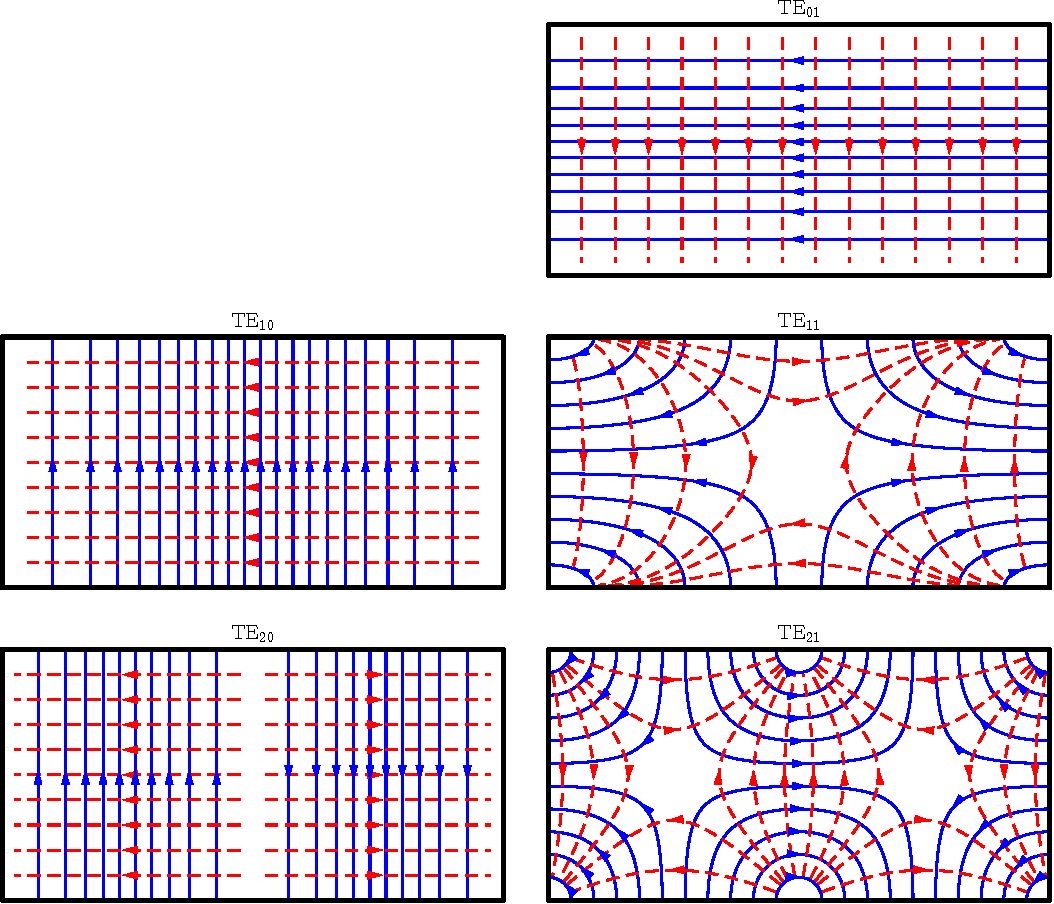
\includegraphics[width=0.8\linewidth]{figures/waveguide_rect_TE.pdf}
    \captionof{figure}{矩形波导的前几个TE模式}
    \label{fig:waveguide rect TE}
\end{notecaptionblock}
可见，TE$_{m0}$模式就是TE$_{10}$模式在$x$方向上复制$m$倍。
同样地，
TE$_{0n}$模式就是TE$_{01}$模式在$y$方向上复制$n$倍；
TE$_{mn}$模式就是TE$_{11}$模式$x$方向上复制$m$倍、在$y$方向上复制$n$倍。

\paragraph{TM模式}
$H_z = 0,\,E_z = \psi$，边界上$\psi = 0$可得
\begin{equation}
    \psi_{mn} = A\sin(k_xx)\sin(k_yy).
\end{equation}
其中$k_x = m\pi/a$，$k_y = n\pi/b$。
截止频率表达式同TE模，但由于$\psi\not \equiv 0$，故$m,n$均不能为0，最低模式为TM$_{11}$。
\begin{subequations}
    \begin{align}
        H_x &= -\i\frac{\omega\varepsilon k_y}{k_\cutoff^2}E_0\sin(k_xx)\cos(k_yy)\e^{\i(k_zz-\omega t)},\\
        H_y &= \i\frac{\omega\varepsilon k_x}{k_\cutoff^2}E_0\cos(k_xx)\sin(k_yy)\e^{\i(k_zz-\omega t)},\\
        H_z &= 0,\\
        E_x &= \i\frac{k_zk_x}{k_\cutoff^2}E_0\cos(k_xx)\sin(k_yy)\e^{\i(k_zz-\omega t)},\\
        E_y &= \i\frac{k_zk_y}{k_\cutoff^2}E_0\sin(k_xx)\cos(k_yy)\e^{\i(k_zz-\omega t)},\\
        E_z &= E_0\sin(k_xx)\sin(k_yy)\e^{\i(k_zz-\omega t)}.
    \end{align}
\end{subequations}
同样地可以画出TM模式在截面上的电场线和磁场线，由于TM$_{mn}$模式同样只是TM$_{11}$模式的简单复制，故只需画出TM$_{11}$模式，如\figref{fig:waveguide rect TM} 所示：
\begin{notecaptionblock}
    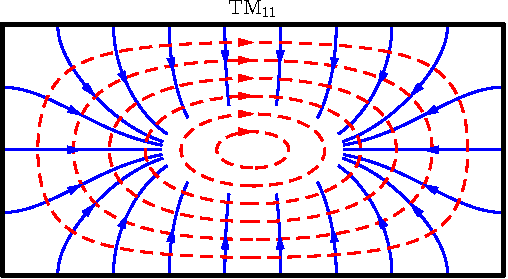
\includegraphics[width=0.4\linewidth]{figures/waveguide_rect_TM.pdf}
    \captionof{figure}{矩形波导的TM$_{11}$模式}
    \label{fig:waveguide rect TM}
\end{notecaptionblock}

\paragraph{传输特性}

取$a > b$，填充真空。TE$_{10}$的截止波长为$2a$，下一个达到截止的模式是TE$_{20}$或TE$_{01}$。取远离两个截止端点的真空波长
\begin{equation}
    \label{eq:ed-rectangular-single-mode-band}
    \max(a,2b) < \lambda < 2a .
\end{equation}
此时只有TE$_{10}$可以把能量带到均匀波导的远处。馈源、台阶或开口附近仍可含有高阶倏逝模。常用的$a = 2b$使第二组模式的截止频率为基模的两倍。

\begin{example}{振荡电偶极能向矩形波导送入多少功率}{waveguide dipole excitation}
    在上述单模波段，将给定偶极矩复振幅$\bm p$的小电偶极放在$(x_0,y_0,0)$，波导两端无限延伸。取时间因子$\e^{-\i\omega t}$，正向TE$_{10}$参考模的横向电场和磁场为
    \begin{align*}
        E_y^+ &= E_{\mathrm{m}}\sin(\pi x/a)\e^{\i k_z z},\\
        H_x^+ &= -E_y^+/Z_{\mathrm{TE}},\qquad Z_{\mathrm{TE}} = \omega\mu_0/k_z .
    \end{align*}
    这里$E_{\mathrm{m}}$是峰值复振幅。对截面上的$\Re(-E_y^+H_x^{+*})/2$积分，参考模沿正向携带的平均功率为$P_{\mathrm{m}} = ab\abs{E_{\mathrm{m}}}^2/(4Z_{\mathrm{TE}})$。

    用\secref{sec:dyadic-green}的互易定理求激发振幅。取反向参考场$\bm E^- = (\bm E^+)^*$、$\bm H^- = -(\bm H^+)^*$，偶极源的电流为$\bm J = -\i\omega\bm p\,\delta^{(3)}(\bm r - \bm r_0)$。对包住偶极的一段波导积分，侧壁上的切向电场为零。两端截面取得足够远，左端的出射场与反向参考模同向，互易定理的两个通量项相消。右端若有振幅$a_+$的正向模，则
    \[
        \int_A(\bm E \times \bm H^- - \bm E^- \times \bm H) \cdot \uvec z\d A
        = -4P_{\mathrm{m}} a_+ = \int\bm E^- \cdot \bm J\d V
        = -\i\omega\bm p \cdot \bm E^-(\bm r_0).
    \]
    因此每一端测到的TE$_{10}$功率均为
    \begin{equation}
        \label{eq:ed-dipole-te10-emitted-power}
        P_+ = P_- = \abs{a_+}^2P_{\mathrm{m}}
          = \frac{\omega^2 Z_{\mathrm{TE}}}{4ab}\abs{p_y}^2\sin^2(\pi x_0/a).
    \end{equation}
    沿$y$放置的偶极在$x_0 = a/2$时耦合最强，沿$x$或$z$放置时该模的激发振幅为零。两端测得的总功率为$2P_+$。
\end{example}

\subsection{圆波导}

圆波导的内半径记为$a$，如\figref{fig:circle waveguide} 所示。
\begin{notecaptionblock}
    \tikzfigure{circle-waveguide}
    \captionof{figure}{圆波导}
    \label{fig:circle waveguide}
\end{notecaptionblock}
采用柱坐标，波动方程\eqref{eqn:laplat+kc2}为：
\begin{equation}
    \Bigp{\pp[2]\rho + \frac1\rho\pp\rho + \frac1{\rho^2}\pp[2]\phi + k_\cutoff^2}\psi = 0,
\end{equation}
分离变量$\psi(\rho,\phi) = R(\rho)\Phi(\phi)$可得
\begin{align*}
    R(\rho) &= AJ_m(k_\cutoff\rho) + BN_m(k_\cutoff\rho),\\
    \Phi(\phi) &= \e^{\pm\i m\phi}.
\end{align*}
其中$J_m,N_m$分别是第一、二类Bessel函数，轴线上场有限，故$B = 0$。
方位角的周期性要求$m$为整数。取$m \geq 0$，对于$m > 0$，$\e^{\i m\phi}$与$\e^{-\i m\phi}$是两个独立的角向解。
以下两幅场线图均取沿 $+z$ 传播的波，纵向场的截面振幅取 $\psi = J_m(k_\cutoff\rho)\cos(m\phi)$。
图中箭头对应 $k_z z - \omega t = -\pi/2$ 的瞬间。对于 $m > 0$，将截面图绕轴旋转 $\pi/(2m)$，就得到角向因子为 $\sin(m\phi)$ 的另一简并模式。

\paragraph{TM模式}

$H_z = 0,\,E_z = \psi$，边界上$\psi = 0$可得
\begin{equation}
    \psi_{mn} = AJ_m(k_\cutoff\rho)\e^{\pm\i m\phi},\quad k_\cutoff = \frac{x_{mn}}a.
\end{equation}
其中$x_{mn}$表示$J_m$的第$n$个正零点。
场的表达式为
\begin{subequations}
    \label{eq:ed-circular-waveguide-tm-components}
    \begin{align}
        H_\rho &= \pm m\frac{\omega\varepsilon}{k_\cutoff^2\rho}E_0J_m(k_\cutoff\rho)\e^{\i(k_zz-\omega t\pm m\phi)},\\
        H_\phi &= \i\frac{\omega\varepsilon}{k_\cutoff}E_0J_m'(k_\cutoff\rho)\e^{\i(k_zz-\omega t\pm m\phi)},\\
        H_z &= 0,\\
        E_\rho &= \i\frac{k_z}{k_\cutoff}E_0J_m'(k_\cutoff\rho)\e^{\i(k_zz-\omega t\pm m\phi)},\\
        E_\phi &= \mp m\frac{k_z}{k_\cutoff^2\rho}E_0J_m(k_\cutoff\rho)\e^{\i(k_zz-\omega t\pm m\phi)},\\
        E_z &= E_0J_m(k_\cutoff\rho)\e^{\i(k_zz-\omega t\pm m\phi)}.
    \end{align}
\end{subequations}

在所选相位，$\bm E_\transv$ 指向 $\psi$ 增大的方向，$\bm H_\transv$ 沿 $\psi$ 的等值线。
如\figref{fig:waveguide circle TM}，轴对称的 TM$_{01}$ 模中，电场线沿半径，磁场线为同心圆。
TM$_{11}$ 模的纵向电场在直径两侧异号，两侧各有一个极值点，极值点处的横向电场为零。图中在这些点附近略微收短电场线，以便分辨相邻曲线。
\begin{notecaptionblock}
    \includegraphics[width=.96\linewidth]{figures/waveguide_circle_TM.pdf}
    \captionof{figure}[圆波导的 TM 模式]{圆波导 TM 模式的横向电场线（深蓝实线）和磁场线（橙色虚线）。在理想导体壁上，横向电场沿壁面法线。}
    \label{fig:waveguide circle TM}
\end{notecaptionblock}

\paragraph{TE模式}

$E_z = 0,\,H_z = \psi$，边界上$\p\psi/\p n = 0$可得
\begin{equation}
    \psi_{mn} = AJ_m(k_\cutoff\rho)\e^{\pm\i m\phi},\quad k_\cutoff = \frac{x_{mn}'}a.
\end{equation}
其中$x_{mn}'$表示$J_m'$的第$n$个正零点。
场的表达式为
\begin{subequations}
    \label{eq:ed-circular-waveguide-te-components}
    \begin{align}
        H_\rho &= \i\frac{k_z}{k_\cutoff}H_0J_m'(k_\cutoff\rho)\e^{\i(k_zz-\omega t\pm m\phi)},\\
        H_\phi &= \mp m\frac{k_z}{k_\cutoff^2\rho}H_0J_m(k_\cutoff\rho)\e^{\i(k_zz-\omega t\pm m\phi)},\\
        H_z &= H_0J_m(k_\cutoff\rho)\e^{\i(k_zz-\omega t\pm m\phi)},\\
        E_\rho &= \mp m\frac{\omega\mu}{k_\cutoff^2\rho}H_0J_m(k_\cutoff\rho)\e^{\i(k_zz-\omega t\pm m\phi)},\\
        E_\phi &= -\i\frac{\omega\mu}{k_\cutoff}H_0J_m'(k_\cutoff\rho)\e^{\i(k_zz-\omega t\pm m\phi)},\\
        E_z &= 0.
    \end{align}
\end{subequations}

在相同相位下，TE 模式的 $\bm H_\transv$ 指向 $\psi$ 增大的方向，$\bm E_\transv$ 沿等值线。
对照\figref{fig:waveguide circle TE} 与\figref{fig:waveguide circle TM}，同为轴对称模式，TE$_{01}$ 模的电场线为同心圆，磁场线沿半径。
\begin{notecaptionblock}
    \includegraphics[width=.96\linewidth]{figures/waveguide_circle_TE.pdf}
    \captionof{figure}[圆波导的 TE 模式]{圆波导 TE 模式的横向电场线（深蓝实线）和磁场线（橙色虚线）。在理想导体壁上，横向磁场的法向分量为零。}
    \label{fig:waveguide circle TE}
\end{notecaptionblock}

\paragraph{前几个$x_{mn}$和$x_{mn}'$分布}

TE和TM的最低模式分别为TE$_{11}$和TM$_{01}$。二者的$k_\cutoff a$分别约为$1.841$和$2.405$，因此圆波导的最低截止模式为TE$_{11}$。
由于$J_0'(x) = -J_1(x)$，TM$_{1n}$和TE$_{0n}$的截止频率相同。

\begin{figure}[H]
    \centering
    \subcaptionbox{$J_m(x)$的零点分布}
        {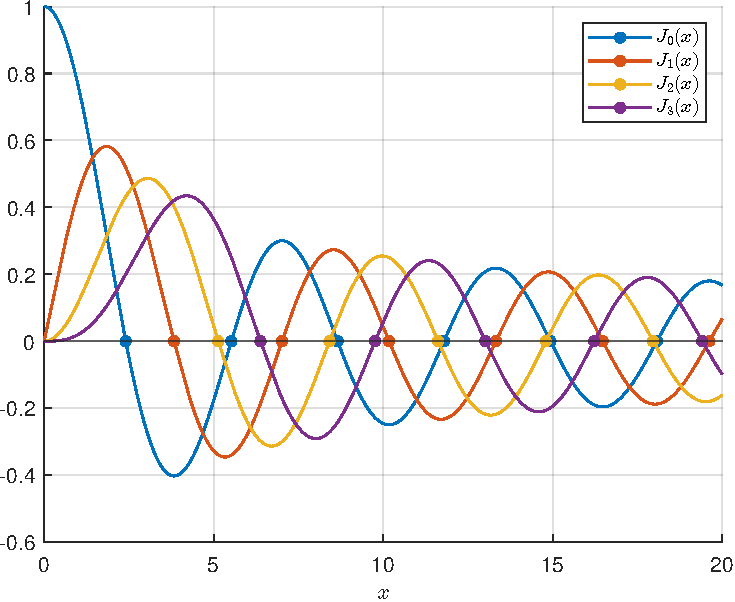
\includegraphics[width=0.45\linewidth]{figures/BesselJzero.pdf}}
    \subcaptionbox{$J_m'(x)$的零点分布}
        {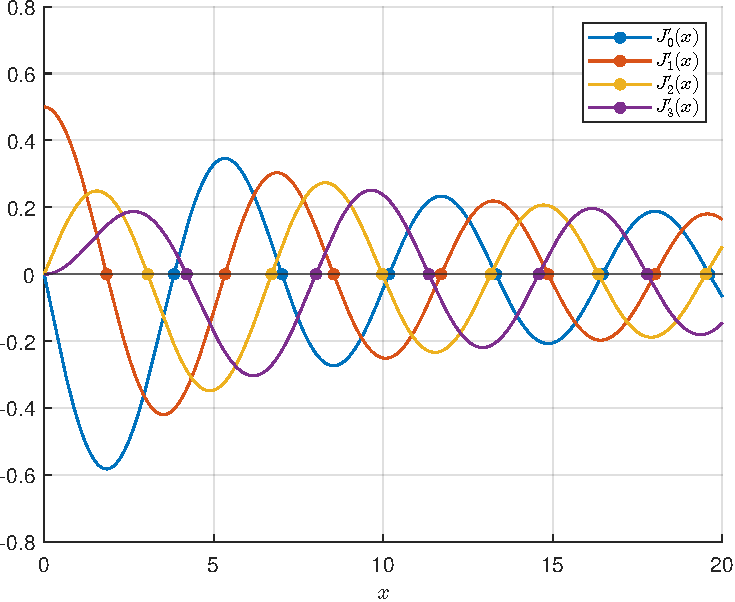
\includegraphics[width=0.45\linewidth]{figures/BesselJpzero.pdf}}
    \caption{$J_m(x)$和$J_m'(x)$的零点分布}
    \label{fig:Bessel function zeros}
\end{figure}

\begin{table}[H]
    \centering
    \caption{$J_m(x)$和$J_m'(x)$的零点}
    \subcaptionbox{$J_m(x)$的零点$x_{mn}$}{
    \begin{tabular}{crrr}
        \toprule
        $x_{mn}$&$n = 1$&$n = 2$&$n = 3$\\
        \midrule
        $m = 0$&2.405&5.520&8.654\\
        $m = 1$&3.832&7.016&10.173\\
        $m = 2$&5.136&8.417&11.620\\
        $m = 3$&6.380&9.761&13.015\\
        \bottomrule
    \end{tabular}}
    \quad
    \subcaptionbox{$J_m'(x)$的零点$x_{mn}'$}{
    \begin{tabular}{crrr}
        \toprule
        $x_{mn}'$&$n = 1$&$n = 2$&$n = 3$\\
        \midrule
        $m = 0$&3.832&7.016&10.173\\
        $m = 1$&1.841&5.331& 8.536\\
        $m = 2$&3.054&6.706& 9.970\\
        $m = 3$&4.201&8.015&11.346\\
        \bottomrule
    \end{tabular}}
\end{table}


\subsection{介质加载波导}

\paragraph{慢波结构}
要让粒子沿波导持续加速，轴向电场须在粒子经过时保持合适的相位，因此轴向相速度应与粒子速度相等。介质加载可降低相速度，同时为粒子保留真空通道。下面用场形较简单的TE模说明介质怎样改变色散关系。TE模的轴向电场为零，纵向加速需要具有$E_z$的模式。
\begin{notecaptionblock}
    \tikzfigure{dielectric-waveguide}
    \captionof{figure}{部分填充介质的矩形波导}
    \label{fig:rectangle waveguide part-filled}
\end{notecaptionblock}
% 后面我们将说明不存在TM模式，
考虑TE模式，根据金属边界条件，两部分的场形式为：
\begin{alignat*}{2}
    H_{z1} &= A\cos(k_{x1}x)\cos(k_{y1}y)\e^{\i k_zz},&k_{y1} &= \frac{n_1\pi}b,\\
    H_{z2} &= B\cos(k_{x2}(a - x))\cos(k_{y2}y)\e^{\i k_zz},&\quad k_{y2} &= \frac{n_2\pi}b.
\end{alignat*}
且
\begin{subequations}
    \begin{align}
        k_{x1}^2 + k_{y1}^2 + k_z^2 = \mu_1\varepsilon_1\omega^2 =: k_1^2,\\
        k_{x2}^2 + k_{y2}^2 + k_z^2 = \mu_2\varepsilon_2\omega^2 =: k_2^2,
    \end{align}
\end{subequations}
由$H_z$在介质分界$x = d$处连续，可得$n_1 = n_2 = n$；当$n \neq 0$时，结合
\[
    H_{yi} = \i\frac{k_z}{k_i^2 - k_z^2}\pv{H_{zi}}y
\]
在$x = d$处连续可知，只要$k_z \neq 0$且$H_z$在界面上不恒为零，就须有$\varepsilon_1\mu_1 = \varepsilon_2\mu_2$。两侧折射率不同时，具有这种横向依赖的一般传播模式同时含有$E_z$和$H_z$。
% 由$E_y,H_y,H_z$在介质分界$x=d$处连续，可得$n_1=n_2=n$且$n\neq 0$时，
但是TE$_{m0}$可以存在，此时$H_y \equiv 0$，再结合
\[
    E_{yi} = -\i\frac{\omega\mu_i}{k_i^2 - k_z^2}\pv{H_{zi}}x
\]
在$x = d$处连续，可得
\begin{equation}
    \frac{\mu_1}{k_{x1}}\sin u\cos v
        + \frac{\mu_2}{k_{x2}}\cos u\sin v = 0.
\end{equation}
这里$u = k_{x1}d$，$v = k_{x2}(a - d)$。
再结合
\begin{equation}
    k_{x1}^2 - k_{x2}^2 = (\mu_1\varepsilon_1 - \mu_2\varepsilon_2)\omega^2,
\end{equation}
便可在给定$\omega$下求得$k_{x1},k_{x2}$和$k_z$。
另一方面，也可以令$k_z = 0$求得截止频率满足的方程：
\begin{equation}
    \sqrt{\frac{\mu_1}{\varepsilon_1}}\sin u_\cutoff\cos v_\cutoff
    + \sqrt{\frac{\mu_2}{\varepsilon_2}}\cos u_\cutoff\sin v_\cutoff = 0.
\end{equation}
其中$u_\cutoff = \omega_\cutoff\sqrt{\mu_1\varepsilon_1}d$、$v_\cutoff = \omega_\cutoff\sqrt{\mu_2\varepsilon_2}(a - d)$。两侧介质相同时，方程化为$\sin(k_xa) = 0$，恢复均匀矩形波导的结果。
若$\mu_1 = \mu_2$、$\varepsilon_1 > \varepsilon_2$且$0 < d < a$，TE$_{m0}$的截止频率位于完全填充两种介质的两个极限之间：
\begin{equation}
    \label{eq:ed-dielectric-guide-cutoff-bounds}
    \frac{m\pi}{a\sqrt{\mu_1\varepsilon_1}} < \omega_\cutoff < \frac{m\pi}{a\sqrt{\mu_2\varepsilon_2}},
\end{equation}

设区域2为真空，电子在其中以速度$v_{\mathrm e}$沿$z$运动。要使电子所见的波相位$k_z z - \omega t$恒定，须有$k_z = \omega/v_{\mathrm e}$。对这里的TE$_{m0}$模，$k_{y2} = 0$，因而
\[
    k_{x2}^2 = \frac{\omega^2}{c^2} - \frac{\omega^2}{v_{\mathrm e}^2}
       = -\frac{\omega^2}{\gamma^2v_{\mathrm e}^2}.
\]
这里$\gamma = (1 - v_{\mathrm e}^2/c^2)^{-1/2}$。
有限能量电子同步时，真空区的横向波数为纯虚数。只有在固定频率取$v_{\mathrm e} \to c$的极限时才有$k_{x2} \to 0$，本征方程中的$\sin v/k_{x2}$相应趋于$a - d$。同步说明粒子能持续处在同一相位；这里的TE模有$E_z = 0$，不能对纯轴向运动的电子做纵向加速功。

\subsection{波导中的能流和衰减}

考虑沿$+z$方向传播的一个TE或TM模。取横截面为$A$，波导内的介质均匀、无耗散且无色散。
复Poynting矢量为
\begin{equation}
    \bm S = \frac12\bm E \times \bm H\conj = \frac{\omega k_z}{2k_\cutoff^4}
    \begin{cases}
        \varepsilon\Bigp{\uvec z\abs{\nabla_\transv\psi}^2 + \i\frac{k_\cutoff^2}{k_z}\psi\nabla_\transv\psi\conj},&\mathrm{TM},\\[1ex]
        \mu\Bigp{\uvec z\abs{\nabla_\transv\psi}^2 - \i\frac{k_\cutoff^2}{k_z}\psi\conj\nabla_\transv\psi},&\mathrm{TE}.
    \end{cases}
\end{equation}
当横向本征函数$\psi$取实数时，第二项是纯虚数，时间平均能流沿$z$方向。
对\eqref{eqn:laplat+kc2}分部积分，边界项因$\psi = 0$（TM模）或$\p\psi/\p n = 0$（TE模）而消失，故
\[
    \int_A\abs{\nabla_\transv\psi}^2\d A = k_\cutoff^2\int_A\abs\psi^2\d A.
\]
取$C = \varepsilon$（TM模）或$C = \mu$（TE模），通过截面的平均功率$P$和单位长度的平均场能量$U$分别为
\begin{subequations}
    \label{eq:ed-waveguide-power-energy}
    \begin{align}
        P &= \int_A\Re\bm S \cdot \uvec z\d A
          = \frac{C\omega k_z}{2k_\cutoff^2}\int_A\abs\psi^2\d A,\\
        U &= \frac14\int_A\bigp{\varepsilon\abs{\bm E}^2 + \mu\abs{\bm H}^2}\d A
          = \frac C2\Bigp{\frac{\omega}{\omega_\cutoff}}^2\int_A\abs\psi^2\d A.
    \end{align}
\end{subequations}
两式相除给出能量沿波导传播的速度
\begin{equation}
    \frac PU = \frac{k_z}{\mu\varepsilon\omega} = \dv\omega{k_z} = v_{\mathrm g}.
\end{equation}
趋近截止时，场仍能储存能量，但单位储能所能输送的功率趋于零。

\paragraph{良导体的波导}
若金属壁的趋肤深度远小于壁厚和截面尺寸，场只进入金属表面一薄层。
由\eqref{eqn:dPloss/da}，波导每单位长度损失的平均功率为
\begin{subequations}
    \label{eq:ed-waveguide-wall-loss}
    \begin{align}
        p_{\mathrm{loss}} &= \frac{R_{\mathrm s}}2\oint_{\p A}\abs{\bm H_\parallel}^2\d\ell,\\
        -\dv Pz &= p_{\mathrm{loss}}.
    \end{align}
\end{subequations}
本节的$\alpha \equiv \alpha_{\mathrm{amp}}$是导模的振幅衰减常数，使场振幅正比于$\e^{-\alpha z}$，则$P(z) = P(0)\e^{-2\alpha z}$。
壁损很小时，积分中的磁场和功率可用理想导体模式的$\bm H^{(0)}$和$P^{(0)}$代入，得到一阶结果
\begin{equation}
    \label{eqn:guide wall attenuation}
    \alpha = \frac{p_{\mathrm{loss}}}{2P^{(0)}}
    = \frac{R_{\mathrm s}}{4P^{(0)}}\oint_{\p A}\abs{\bm H^{(0)}_\parallel}^2\d\ell .
\end{equation}
分子取沿金属表面的全部磁场分量，包括纵向磁场$H_z$。若填充介质也有微弱吸收，每单位长度的损失还应加上$\textstyle \int_A q_{\mathrm{abs}}\d A$，其中$q_{\mathrm{abs}}$按理想模式的场计算。总功率损失除以$2P^{(0)}$给出总振幅衰减常数；同一导模的功率衰减常数则是它的两倍。

\paragraph{矩形波导的最小衰减频率}
以$a \times b$矩形波导的TE$_{10}$模为例。记$k_\cutoff = \pi/a$，则$H_z = H_0\cos(k_\cutoff x)$，
$H_x = -\i(k_z/k_\cutoff)H_0\sin(k_\cutoff x)$，二者省略了共同的传播因子。
在$x = 0,a$的两面上只需计入$H_z$，在$y = 0,b$的两面上则两个分量都要计入。于是
\begin{align*}
    \oint_{\p A}\abs{\bm H^{(0)}_\parallel}^2\d\ell
       &= \abs{H_0}^2\Bigb{2b + a\Bigp{1 + \frac{k_z^2}{k_\cutoff^2}}},\\
    P^{(0)} &= \frac{\mu\omega k_z ab}{4k_\cutoff^2}\abs{H_0}^2.
\end{align*}
记填充介质的本征阻抗$\eta = \sqrt{\mu/\varepsilon}$，代入\eqref{eqn:guide wall attenuation}得
\begin{equation}
    \alpha_{10} = \frac{R_{\mathrm s}}{\eta b}\,
    \frac{1 + (2b/a)(\omega_\cutoff/\omega)^2}{\sqrt{1 - (\omega_\cutoff/\omega)^2}}.
\end{equation}
在截止附近，同样的壁电流对应较小的输送功率，因而衰减急剧增大。
在高频端，正常趋肤效应给出$R_{\mathrm s} \propto \sqrt\omega$，衰减也随之上升。
例如$a = 2b$，令$x = \omega/\omega_\cutoff$，则$\alpha_{10} \propto (x^2 + 1)/\sqrt{x(x^2 - 1)}$。
令导数为零，得$x^4 - 6x^2 + 1 = 0$，在传播区间内的极小值位于$x = 1 + \sqrt2$。
此时已超过第二个模式的截止频率$2\omega_\cutoff$，这个极小值描述单独激发的TE$_{10}$模。

\section{边界条件的扰动}
功率损失给出振幅衰减。要同时求相位的变化，需要保留金属壁上切向电场与磁场的相位差。
沿用从金属指向波导内部的法向量$\uvec n$，前面求出的良导体表面场满足
\begin{equation}
    \bm E_\parallel = Z_{\mathrm s}\uvec n \times \bm H_\parallel,
    \qquad Z_{\mathrm s} = (1 - \i)R_{\mathrm s}.
\end{equation}
$Z_{\mathrm s}$称为表面阻抗(surface impedance)，虚部的符号对应于时间因子$\e^{-\i\omega t}$。

在同一个实频率下，记理想壁模式为$(\bm E^{(0)},\bm H^{(0)})$，其纵向波数为$k_z$。
良导体壁上的相应模式记作$(\bm E,\bm H)$，纵向波数为$k_z + \Delta k_z$。
在波导内部用Maxwell方程展开散度，可得
\begin{align*}
    \div\bm F &= 0,\\
    \bm F &= \bm E \times \bm H^{(0)\ast} + \bm E^{(0)\ast} \times \bm H .
\end{align*}
对波导的一薄段应用散度定理。$\bm F$随$z$按$\e^{\i\Delta k_z z}$变化，
侧壁处的外法向为$-\uvec n$，理想壁的切向电场为零，故
\[
    \i\Delta k_z\int_A\bm F \cdot \uvec z\d A
    = -\oint_{\p A}Z_{\mathrm s}\bm H_\parallel \cdot \bm H^{(0)\ast}_\parallel\d\ell .
\]
两端的积分都已乘上一阶小量，可在积分中代入理想壁的场。左端的截面积分等于$4P^{(0)}$，于是
\begin{equation}
    \Delta k_z \simeq \frac{\i Z_{\mathrm s}}{4P^{(0)}}
        \oint_{\p A}\abs{\bm H^{(0)}_\parallel}^2\d\ell = (1 + \i)\alpha .
\end{equation}
因此场沿轴的因子为$\e^{\i(k_z+\alpha)z}\e^{-\alpha z}$。虚部给出了由能量守恒所得的衰减，实部说明波导波长略有缩短。
上述微扰要求$\abs{\Delta k_z} \ll k_z$，在十分接近截止处须重新求解有损模式。
遇到简并模式时，应先在简并子空间内选取使壁面磁场重叠积分对角化的功率归一化模式。

\section{谐振腔}
将一段长$d$的波导在$z = 0,d$处用理想金属端板封闭。前进波和反射波叠加成驻波，
端面上的切向电场和法向磁场均为零，故纵向分量分别取
\begin{align*}
    \mathrm{TM}&:&E_z = \psi(x,y)\cos\Bigp{\frac{p\pi z}d},&&p &= 0,1,2,\ldots,\\
    \mathrm{TE}&:&H_z = \psi(x,y)\sin\Bigp{\frac{p\pi z}d},&&p &= 1,2,3,\ldots.
\end{align*}
横截面决定$k_\cutoff$的允许值，端面间距决定纵向波数$p\pi/d$。相应的本征频率为
\begin{equation}
    \omega_p^2 = \frac1{\mu\varepsilon}\Bigb{k_\cutoff^2 + \Bigp{\frac{p\pi}d}^2}.
\end{equation}
同一横截面模式可有多个纵向驻波。TM模还允许$p = 0$，此时轴向电场处处垂直于端面，频率与腔长无关。

\section{腔内的功率损失}
腔内的驻波也在金属表面激起电流。取均匀、无色散的填充介质，对一个孤立的本征模式，
电场和磁场的时间平均总能量相等。因此总储能$W$和整个内壁上的平均损耗功率分别是
\begin{subequations}
    \label{eq:ed-cavity-energy-wall-dissipation}
    \begin{align}
        W &= \frac14\int_V\bigp{\varepsilon\abs{\bm E}^2 + \mu\abs{\bm H}^2}\d V
          = \frac\mu2\int_V\abs{\bm H}^2\d V,\\
        P_{\mathrm{loss}} &= \frac{R_{\mathrm s}}2\oint_{\p V}\abs{\bm H_\parallel}^2\d a.
    \end{align}
\end{subequations}
其中的场取理想腔模。只有壁损时，品质因子(quality factor)可由下式求得
\begin{equation}
    \label{eqn:cavity wall Q}
    Q = \omega_0\frac W{P_{\mathrm{loss}}}
      \simeq \frac{\omega_0\mu}{R_{\mathrm s}}\,
      \frac{\displaystyle\int_V\abs{\bm H}^2\d V}
           {\displaystyle\oint_{\p V}\abs{\bm H_\parallel}^2\d a}.
\end{equation}
这里$\omega_0$为谐振角频率，积分范围包括两块端板和侧壁。
切断激励后，由$\d W/\d t = -P_{\mathrm{loss}}$得
\begin{equation}
    \label{eq:ed-cavity-ringdown}
    W(t) = W(0)\e^{-\omega_0 t/Q},\qquad
    E_{\text{包络}}(t) \propto \e^{-\omega_0 t/(2Q)}.
\end{equation}
对于$Q \gg 1$的孤立共振，将这个指数衰减的振荡作Fourier变换，得到共振附近的功率线形
\begin{equation}
    \label{eq:ed-cavity-power-lineshape}
    \abs{E(\omega)}^2 \propto
       \frac1{(\omega - \omega_0)^2 + (\omega_0/2Q)^2}.
\end{equation}
两个半功率点之间的角频率差为$\Delta\omega = \omega_0/Q$。若腔还通过耦合口向外输出功率，
求测得的线宽时应将输出功率也计入总损耗。

\paragraph{圆柱腔的TM$_{010}$模}
取半径$a$、长$d$的真空腔，壁材料无磁性。记$x_{01} \simeq 2.405$为$J_0$的第一个正零点。
由圆波导TM模取$p = 0$，得到$\omega_0 = c x_{01}/a$，且仅有两个场分量
\begin{equation}
    \label{eq:ed-tm010-fields}
    E_z = E_0J_0(x_{01}\rho/a),\qquad
    H_\phi = -\i\frac{E_0}{Z_0}J_1(x_{01}\rho/a).
\end{equation}
$H_\phi$在侧壁和端板上均为切向分量。利用Bessel函数的积分恒等式
\[
    \int_0^a\rho J_1^2(x_{01}\rho/a)\d\rho = \frac{a^2}{2}J_1^2(x_{01}),
\]
记$H_a = \abs{H_\phi(a)}$，体积积分和壁面积分分别为
\begin{align*}
    \int_V\abs{\bm H}^2\d V &= \pi a^2d H_a^2,\\
    \oint_{\p V}\abs{\bm H_\parallel}^2\d a &= 2\pi ad H_a^2 + 2\pi a^2 H_a^2.
\end{align*}
右端两项依次来自侧壁和两块端板。由$R_{\mathrm s} = \mu_0\omega_0\delta/2$，\eqref{eqn:cavity wall Q}给出
\begin{equation}
    Q_{010} = \frac{ad}{(a + d)\delta}.
\end{equation}
在固定半径下缩短腔长，谐振频率保持不变。储能与腔长成正比，而两块端板的损耗在固定场幅下保持不变，因此短腔的线宽变大。\secref{sec:single cavity mode}将用同一场分布算出腔内一个光子对应的电场振幅。
